% !TeX root = ../Bachelorarbeit.tex
\chapter{Prototypischer Lösungsansatz}
\section{Implementationsdetails}
\begin{enumerate} 
\item \textbf{Client / Webseite}

Die Webseite besteht aus einer zur \ac{spa} ähnlichen Architektur, die ausschließlich Javascript und JQuery, also clientseitige Programmiersprachen nutzt. SPA's sind Webapplikationen, bei denen der Nutzer eine Seite betritt und diese nie wieder vollständig laden muss. Frameworks wie Angular, React oder VueJS basieren auf dieser Mechanik und nutzen Javascript und JQuery um die Ladezeiten einer Webseite durch Module zu reduzieren. Anstatt also die gesamte Webseite neuzuladen, laden diese Frameworks nur spezielle Bereiche der Webseite asynchron nach. In dem Prototyp ist dies nur größtenteils der Fall, da neben der Hauptseite \textbf{index.html} eine weitere Seite existiert, auf die man bei erfolgreichem Login weitergeleitet wird: \textbf{secret\_panel.html}. Auch werden keine Module nachgeladen, sondern bei entsprechender Aktion nur Elemente innerhalb des DOM - Baums per id identifiziert und versteckt.

Beim Betreten von beiden Seiten der Anwendung findet eine Prüfung nach dem Session-Cookie (\textbf{user\_sid}) statt, die vom Server bei einer erfolgreichen Authentifikation im Header über 'Set-Cookie' als Response zurückkommt und vom Browser infolge dessen gesetzt wird. Der Aufruf der \textbf{index.html} Seite ist nicht möglich mit gesetztem Cookie und leitet den User auf \textbf{secret\_panel.html} weiter und umgekehrt genauso. Die Sicherung dieses Cookies auf Serverseite durch Prüfungen ist nicht Bestandteil dieser Arbeit, hier wird sich lediglich auf den Loginprozess von Anwendungen konzentriert um dessen Schwächen und die Vorteile neuer Verfahren aufzuzeigen. Aktuell könnte ein Angreifer demnach selbst einen entsprechenden Cookie mit einem Wert setzen und das 'geheime Panel' erreichen. Bei weiter ausgereiften Webapplikationen wird bei jedem Request an den Server der Session Cookie mit einer temporären Map innerhalb des Backends abgeglichen. Befindet sich der Session Cookie nicht in dieser Map oder hat nicht genügend Rechte für diese Anfrage, erhält der Nutzer den Statuscode 401 (Unauthorized) zurück. So haben es etablierte Dienste wie 'Netflix' bereits umgesetzt.

Aus der Forschungsfrage ergibt sich, dass die Webseite ausschießlich Javascript (oder auf Javascript basierende Programmiersprachen wie JQuery) zur Implementation der Programmlogik verwendet. Javascript selbst ist eine clientseitige Programmiersprache und gibt dem Nutzer den gesamten Code auf Webseiten preis. Demnach wurde bei der Anwendung darauf geachtet, alle clientseitigen Prüfungen, auch serverseitig zu implementieren. Zumindestens alle wichtigen Prüfungen, die sonst den Programmablauf verhindern würden oder sogar Serverabstürze zur Folge hätten. Nicht nur gibt Javascript den Code preis, über die Konsole (Unter Google Chrome und Firefox in den Entwickleroptionen des Browsers zu finden) lassen sich ganze Funktionen oder globale Variablen manipulieren. Variablen innerhalb von Funktionen können vom Angreifer nicht so leicht manipuliert werden.

Möglich ist es dennoch, den Inhalt dieser Funktion in eine andere Funktion zu schreiben, um die Variable dort auszutauschen. Um dem Nutzer nicht jede Funktion problemlos erreichbar zu machen, wurde bei der Implementation das Revealing-Module-Pattern angewendet, über die gewisse Variablen nicht im globalen Scope (window) sondern im Scope einer Funktion bleiben, die nur gewisse andere Funktionen in sich exportiert und als eine Art Schnittstelle fungiert. \\\\

\begin{figure}[ht]
	\centering
	\animategraphics[width=\linewidth]{12}{webapp_design/frame-}{0}{121}
	\caption[Design des Prototypen (Codename: clsec)]{Design des Prototypen (Codename: clsec) - Anklicken zum Abspielen}
	\label{fig:webapp_design}
\end{figure}
\newpage

Das Design der Webanwendung ist kein wesentlicher Punkt dieser Arbeit und deshalb schlicht gehalten. So besteht der Prototyp aus einer einfachen Webseite, die aus dem globalen Internet erreichbar ist und die zwei Eingabefelder und einen Loginbutton besitzt. Um sich die Designarbeit oder das Suchen von Icons und passenden Buttondesigns zu sparen wurde auf bekannte Frameworks wie Bootstrap4 und Funktionalitäten wie Flexbox gesetzt, das ein automatisches Rescaling und Positioning von Webseitenelementen umsetzt. So war es nicht nötig ein Loginformular zu designen sondern vorhandene Strukturen von Bootstrap für Buttons aller Art zu nutzen. Die unterschiedlichen Methoden der Authentifizierung wählt man über ein Dropdownmenü über dem Login - Button. Je nach Authentifizierungsverfahren werden andere Elemente sichtbar, die die weiteren Schritte für die Authentifikation erläutern. Die Methode kann sowohl über das Dropdownmenü als auch über einen Klick auf die Pfeile links und rechts neben dem Dropdownmenü gewählt werden. Dabei wurde eine Art Pagination zwischen den verschiedenen behandelten Verfahren umgesetzt. Ist man am Ende der drei Methoden, springt man wieder zur ersten Methode und andersherum.

Bei der Web Authentication gibt es eine Besonderheit. Die Webseite muss auf die Schnittstellen des Betriebssystems zugreifen, um den Nutzer zu verifizieren. Dieser Teil kann von dem Prototyp nicht beeinflusst werden und wird vom \ac{ctap}2 Protokoll innerhalb des FIDO2 Standards definiert. Dadurch entstehen teilweise merkwürdige und aus UX (User Experience) - Sicht höchst fragwürdige Interaktionen. So fragt das Betriebssystem zunächst (bei entsprechender Möglichkeit) nach einem PIN um den Nutzer zu registrieren. Drückt man nun die Escape-Taste erscheint ein Dialog um einen Sicherheitsschlüssel (ein externes Gerät) einzurichten. Beim Login wiederrum ist dies durch eine Dropdownliste schöner gelöst worden, wo der User alle möglichen Loginmethoden auf einem Blick sieht und diese Wählen kann. Während er bei der Registration keine Chance hat dies zu tun und immer erst ein PIN - Feld angezeigt wird. Auf die einzelnen behandelten Verfahren wird in späteren Kapiteln noch genauer eingeggangen, da werden solche Schwierigkeiten aufgegriffen da dies nur eines von vielen 'Problemen' neuerer Verfahren ist: Die Abhängigkeit vom Betriebssystem.

\item \textbf{Server}

Der NodeJS - Server besteht aus einer REST Api, die keine Zustände speichert. Neben der Aufgabe des Cookie Managements und der Generierung von UUID's liefert er zudem die Schnittstelle zur Datenbank und verschiedene Funktionalitäten für die behandelten Verfahren Username \& Passwort, \ac{totp} und Webauthn:

\begin{itemize}
 \item \textbf{/logout} - POST - Löscht den Session-Cookie (und damit die Session des Nutzers) und leitet ihn auf die Loginseite \textbf{index.html} weiter.

 \item \textbf{/get\_public\_key} - GET - Liest den öffentlichen Schlüssel des Servers ein und gibt diesen in einer JSON - Struktur zurück. Ist wichtig für die Username \& Passwort - Authentifizierung.

 \item \textbf{/password/login} - POST - Nimmt einen mit dem öffentlichen Schlüssel des Servers verschlüsselten Usernamen und Passwort entgegen und entschlüsselt diese mit dem privaten Schlüssel. Im Anschluss darauf wird in der Datenbank über eine gepoolte Query nach dem Nutzer gesucht. Wurde dieser gefunden, erstellt der Server einen SHA512 - Hash aus dem Passwort (aus dem Request) und dem Salt des Users (aus der Datenbank) indem die \textbf{hashString} - Methode aufgerufen wird. Diese bezieht den Pepper des Servers mit ein. Sofern die Hashes aus der Datenbank und der soeben Generierte übereinstimmen, erhält der Nutzer die Response 200 und den Text ``OK''. Gleichzeitig wird wie bei jeder anderen Authentifizierungsmethode die \textbf{createSessionCookie} - Methode aufgerufen um den Session-Cookie (eine zufällige UUID) im Header zurück an den Nutzer zu senden, sodass dessen Browser ihn setzt..
 \newpage
 
 \item \textbf{/password/create\_password\_hash} - GET - Nimmt eine Zeichenkette des Nutzers entgegen und erstellt einen Password-Hash für den Nutzer, der manuell in die Datenbank persistiert werden kann. Ist als 'Quality of Service' Funktion zu verstehen, um es dem Administrator einfacher zu machen, Passwörter zu erstellen, die bei Vergleich einen gülltigen Hash ergeben.
 
 \item \textbf{/totp/check\_username} - POST - Diese Methode dient lediglich der Prüfung, ob der Nutzer die \ac{totp} Authentifikation mittels zufälligem SECRET bereits gegenüber der Webseite validiert hat. Das Datenbankfeld 'totp\_activated' wird hier geprüft, ist der Wert 1 (für das boolsche 'wahr') liefert der Server den Text ``Success'' zurück, das der Client deutet um nur das Feld für den sechsstelligen TOTP Code anzuzeigen. Hat das Feld allerdings den Wert 0, wird (sofern noch nicht vorhanden im Feld 'totp\_secret') ein neues Secret erstellt und in der Datenbank für diesen Nutzer persistiert. Gleichzeitig wird eine URL beginnend mit otp:// erstellt, um diesen zusammen mit einem Base64 enkodierten QR Code an den Client zu schicken, der dies dem User präsentiert. Es wurde sich hier bewusst dazu entschieden, diese Schritte auf Serverseite vorzunehmen. Möglich wäre es auch auf Clientseite gewesen, wäre aber durch die Suche nach passenden Javascript Modulen mit einem Mehraufwand verbunden gewesen, welches verhindert werden sollte.
 
 \item \textbf{/totp/check\_token} - POST - Nimmt den Usernamen des Nutzers und einen sechsstelligen \ac{totp} Token entgegen. Sucht im Anschluss darauf in der Datenbank nach dem Nutzer und prüft über die Library 'otplib' ob der eingegebene \ac{totp} - Token zum secret in der Datenbank valide ist. Dieser Schritt findet sowohl bei der Registration als auch beim Login statt. Wenn das Feld 'totp\_activated' also 0 ist, wird es bei der ersten Authentifikation auf 1 gesetzt und der Nutzer wird eingeloggt. (Session-Cookie wird gesetzt und Nutzer weitergeleitet)
 \newpage

 \item \textbf{/webauthn/generate-attestation-options} - POST
 Liefert dem Nutzer die verschiedenen Registrieroptionen für die Web Authentication mittels WebauthnAPI. Dabei wurden verschiedene Optionen gesetzt, die im folgenden erklärt werden und die der User im Body der Response als JSON - Objekt erhält. Zur Vereinfachung werden hier nur die Optionen aus der abstrahierten Library und dessen Möglichkeiten erklärt. Dies ist zum Verständnis der Arbeit und des Prototypen ausreichend.
 
 \begin{lstlisting}[language=json,firstnumber=1]
        {
            rpName: 'clsec',
            rpId: 'localhost',
            userID: 4,
            userName: 'username',
            userDisplayName: 'username',
            attestationType: 'none',
            authenticatorSelection: {
                requireResidentKey: false,
                userVerification: "discouraged",
            },
            excludedCredentialIDs: userAuthenticators.map(dev => dev.credentialID),
        }
\end{lstlisting}

\textbf{rpName:} rp steht hier bei für Relying Party. Das ist der Name, der später auch im Registrierungsdialog als 'Webseiteninhaber' gelistet wird.

\textbf{rpId:} Die Relying Party Id ist eine URL, auf der sich der Nutzer registrieren möchte. In unserem Falle ist dies 'localhost' ohne Zusätze wie das Protokoll oder der Port. Diese Variable ist vor allem für Webseiten im Netz wichtig, sodass ein Angreifer nicht per Pishing den Nutzer zur Registrierung auf einer anderen Webseite bringt. Die Registrierung schlägt clientseitig fehl, wenn die rpId und die Webseitenaddresse (Damit ist nicht die Domain sondern die wahrliche IP-Addresse gemeint) nicht übereinstimmen. Beim Wert 'localhost' sendet der Server diesen Teil der JSON - Abfrage nicht mit, da es localhost aus Testgründen nicht prüft. Gleichzeitig erzwingt Webauthn ausschließelich für diese rpId keine sichere Verbindung.

\textbf{userID:} Das ist die ID des Nutzers die verifiziert wird, meist eine fortlaufende Ganzzahl.

\textbf{userDisplayName:} Das ist der Name, der beim Registrieren als Username gelistet wird.

\textbf{attestationType:} Der Server definiert, wie viele Informationen über den Authenticator er im attestation statement haben möchte. Das attestation statement erhält er nach dem der User sich mit einem Authenticator registriert hat und ist ein wichtiger Bestandteil des Objekts welches den Server im Nachhinein über eine erfolgreiche Registration benachrichtigt. Ferner ist der öffentliche Schlüssel des Nutzers in diesem Objekt lokalisiert, den der Server dann in der Datenbank persistiert. 'none' bedeutet hierbei, dass keinerlei Informationen erwünscht sind. 'indirect' als Option würde dem Nutzer erlauben selbst zu entscheiden wie viele Informationen er preisgibt bzw. könnte er eine anonymisierte CA verwenden um sein Zertifikat auszustellen und 'direct' als Option würde die Daten direkt vom Authenticator ohne einen Eingriff des Nutzers erwarten.

\textbf{authenticatorSelection:} Das sind verschiedene Optionen um den verwendeten Authenticator zu bestimmen. Das Argument 'requireResidentKey' bestimmt hierbei darüber, ob ein Authenticator benutzt werden darf, der selbst nicht in der Lage wäre einen privaten Schlüssel auf dem Betriebssystem zu sichern und dem Server infolge dessen einen öffentlichen Schlüssel zu senden. Die 'userVerification' ist im Prototyp nicht erzwungen also 'required' sondern 'discouraged', es obliegt also dem Betriebssystem und dem zu authentifizierenden Gerät / und der initialen Konfiguration zu entscheiden, ob der Nutzer sich gegenüber seines Authenticators verifizieren muss. In dem Beispiel eines bereits sicheren FIDO2 - USB Sticks könnte dies zum Beispiel nicht vom Nutzer gewünscht sein.

\textbf{excludedCredentialIDs:} Dies ist eine Liste von credentialID's die in der Datenbank im Feld 'webauthn\_authenticator\_data' als JSON - Struktur persistiert sind. Sie dient dazu, bereits registrierte Methoden nicht erneut anzuzeigen, funktioniert dennoch nicht zuverlässig.
\end{itemize}
\newpage

\item \textbf{Datenbank}

Das gewählte Datenbankmanagementsystem ist PosgreSQL 12, dies hat einen speziellen Grund. Das Datenbankmanagementsysten besitzt fortgeschrittene Funktionalitäten um JSON Strukturen zu persistieren und zu bearbeiten. Gleichzeitig wäre es möglich Constraints zu erstellen, die bei anderen Managementsystemen wie MYSQL nur bei speziellen Tabellentypen wie InnoDB und das auch nicht vollständig verfügbar sind. Der Prototyp benötigt nur eine einzige Tabelle namens \textbf{users}, dessen Struktur anhand des folgenden SQL Statements erläutert wird.\\

 \begin{lstlisting}[language=sql,firstnumber=1]
CREATE TABLE public.users
(
    id bigint NOT NULL,
    username text COLLATE pg_catalog."default" NOT NULL,
    password text COLLATE pg_catalog."de-DE-x-icu" NOT NULL,
    salt text COLLATE pg_catalog."default",
    totp_secret text COLLATE pg_catalog."default",
    totp_activated integer NOT NULL DEFAULT 0,
    webauthn_register_challenge text COLLATE pg_catalog."default" NOT NULL DEFAULT ''::text,
    webauthn_login_challenge text COLLATE pg_catalog."default" NOT NULL DEFAULT ''::text,
    webauthn_authenticator_data jsonb,
    CONSTRAINT users_pkey PRIMARY KEY (id)
)
\end{lstlisting}

Er speichert typische Daten um den Nutzer zu authentifizieren. Jeder Nutzer besitzt eine eigene einzigartige ID, die eine Ganzzahl ist. Dann besitzt jeder User einen Nutzernamen im Feld 'username'. Die Felder 'password' und 'salt' besitzen logischerweise nur Nutzer, die die Passwort Authentifikation unterstützen. Die Felder 'totp\_secret' und 'totp\_activated' werden einerseits genutzt um das Geheimnis (welches der User beim TOTP Setup einscannt) zu erstellen und den Nutzer damit später zu authentifizieren und andererseits um dem Frontend zu signalisieren, ob der Nutzer das Setup vollzogen hat. Die Challenge-Felder für Webauthn 'webauthn\_register\_challenge' und 'webauthn\_login\_challenge' sind als eine Art Zwischenablage zu verstehen und hätten theoretisch auch im Cache des Backends persistiert werden können, da bei jeder neuen Registration und jedem neuen Login durch Webauthn eine neue Challenge vom Server erstellt und vom Nutzer nach dem Signieren zurückkommt. Interessant ist das Feld 'webauthn\_authenticator\_data', das in einer JSON-Liste alle registrierten Geräte für die Web Authentication beinhält.
\newpage

 \begin{lstlisting}[language=json,firstnumber=1]
[
    {
        "counter": 0,
        "publicKey": "pAEDAzkBACBZAQCgna71QX...",
        "credentialID": "HEeJWgh9QOWURee7dF..."
    },
    {
        "counter": 2,
        "publicKey": "pQECbt1via1qrycev0vyc...",
        "credentialID": "_HbcWx_XWd6Pyjyh..."
    },
    {
        "counter": 5,
        "publicKey": "pQECAyYgASFYIGpEwj...",
        "credentialID": "45nEVRuXWky8CyvW79e..."
    }
]
\end{lstlisting}

Dabei besitzt jedes Element jeweils einen counter, um die Anzahl an Einloggversuchen zu zählen, den öffentlichen Schlüssel und eine einmalige credentialID, die bei jeder Registration als 'exludedCredentialID' an den Clienten übermittelt wird, um zu signalisieren das diese credentialID sich nicht erneut registrieren kann. (Um doppelte Registrationen von ein und dem selben Gerät zu verhindern für den selben Nutzer)
\end{enumerate}

\section{Fehlerbetrachtung}

Die Fehlerbetrachtung ist essenziell um nun auf die Probleme einzugehen, die während der Implementation bereits ersichtlich wurden.

\begin{enumerate}
\item \textbf{UX-Probleme bei Geräteregistrierung für Webauthn unter Windows}

Bei der Implementation des Webauthn - Protokolls schien es zunächst ein Mal nicht ersichtlich ob die unerklärlichen Dialogboxen nun ein Implementationsproblem darstellten oder tatsächlich so gewollt sind. Erst die Prüfung durch das offizielle 'Playground-Tool' der FIDO Alliance, zu finden unter 'https://webauthn.io/' wurde es ersichtlich, dass die verwirrenden UX Entscheidungen von Windows kein Fehler des Prototyps sind. 
\newpage

Dennoch tragen sie zur allgemeinen Unverständnis bei.
Bei diesem Problem geht es um folgende Abfolge an Dialogboxen, die bei der Registration eines neuen Geräts erscheinen:

\begin{enumerate}
\item Der Nutzer klickt unter Angabe seines Nutzernamens auf den Button 'Gerät registrieren' und erwartet eine Auswahl an vorhandenen Geräten, die registriert werden können. In diesem Beispiel stehen ein physischer Sicherheitsschlüssel und Windows-Hello-PIN zur Verfügung.

\begin{figure}[ht]
	\centering
	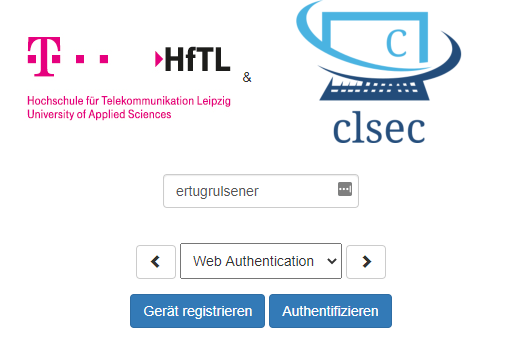
\includegraphics[width=8cm]{ux_problem_1.png}
	\caption[UX-Problem bei Webauthn Geräteregistrierung (1)]{UX-Problem bei Webauthn Geräteregistrierung (1)}
	\label{fig:ux_problem_1}
\end{figure}

\item Statt der erwarteten Auswahlbox erhält der Nutzer die Möglichkeit auf die Windows-Hello-PIN und geht nicht von weiteren Auswahlmöglichkeiten aus.

\begin{figure}[ht]
	\centering
	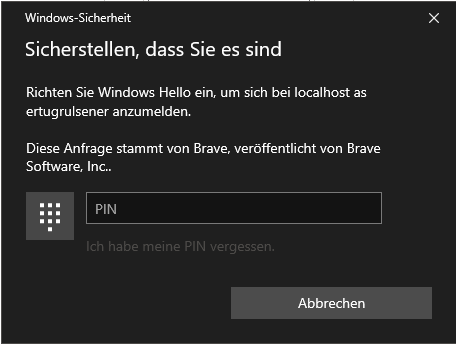
\includegraphics[width=8cm]{ux_problem_2.png}
	\caption[UX-Problem bei Webauthn Geräteregistrierung (2)]{UX-Problem bei Webauthn Geräteregistrierung (2)}
	\label{fig:ux_problem_2}
\end{figure}
\newpage

\item Beim Betätigen der Escape-Taste erscheint plötzlich der Dialog, um einen Sicherheitsschlüssel zu registrieren. Dies ist bereits ein Problem, weil der User sich zum Zeitpunkt der Registration nicht über diese Möglichkeit bewusst ist. Bei der Implementation ist diese Option auch nur durch Zufall aufgefallen.

\begin{figure}[ht]
	\centering
	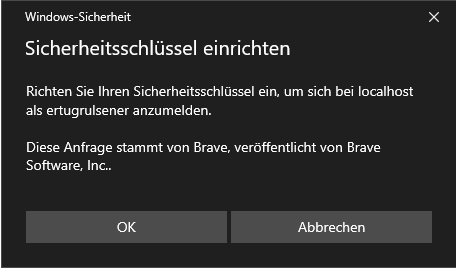
\includegraphics[width=8cm]{ux_problem_3.png}
	\caption[UX-Problem bei Webauthn Geräteregistrierung (3)]{UX-Problem bei Webauthn Geräteregistrierung (3)}
	\label{fig:ux_problem_3}
\end{figure}

\item Im Vergleich dazu sieht der Dialog für den Login, wie vom Nutzer erwartet, durch ein Gerät folgend aus (sofern das Feld 'webauthn\_authenticator\_data' nicht leer ist):

\begin{figure}[ht]
	\centering
	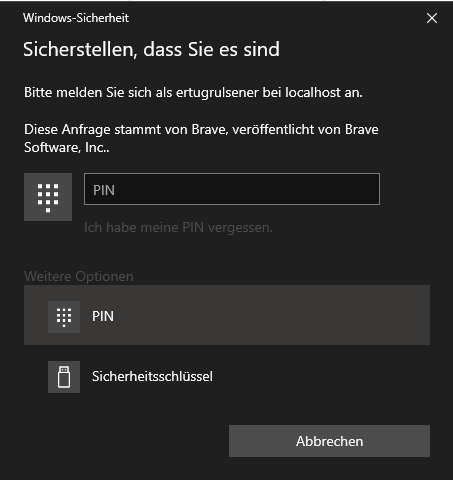
\includegraphics[width=8cm]{ux_problem_4.png}
	\caption[UX-Problem bei Webauthn Geräteregistrierung (4)]{UX-Problem bei Webauthn Geräteregistrierung (4)}
	\label{fig:ux_problem_4}
\end{figure}
\end{enumerate}
\newpage

\item \textbf{Unerwartete Auswahlmöglichkeiten bei keinem registrierten Authenticator}

Sollte das Feld 'webauthn\_authenticator\_data' allerdings leer sein, erscheint folgender Dialog:

\begin{figure}[ht]
	\centering
	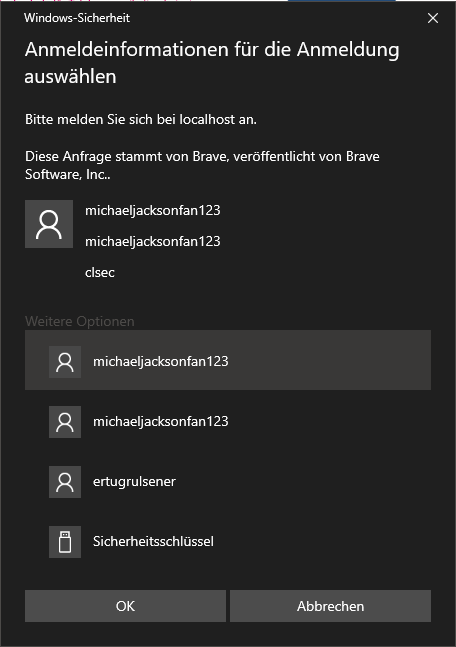
\includegraphics[width=8cm]{ux_problem_5.png}
	\caption[UX-Problem bei Webauthn Geräteregistrierung (5)]{UX-Problem bei Webauthn Geräteregistrierung (5)}
	\label{fig:ux_problem_5}
\end{figure}

Dieser ist insofern ein Fehler, da kein Sicherheitsschlüssel registriert wurde und bei Auswahl dessen nichts passiert. Gleichzeitig werden hier von Windows alle erstellten 'Profile' während der Testphase angezeigt, dessen Name gleich verwirrend für den Nutzer ist. Wenn also das Profil mit dem Namen 'michaeljacksonfan123' versucht einzuloggen, erhält er einen Statuscode 401 (Nicht autorisiert) als Response. Der Fehler hierbei ist die Anzeige einer Einloggoption durch Windows-Sicherheit, die nicht valide ist. Selbst bei bestätigtem und korrektem PIN. Die Felder 'exludedCredentialIDs' für die Registration und 'allowedCredentialIDs' für den Login scheinen keine Wirkung zu zeigen, dies könnte einerseits an der WebauthnAPI liegen, die ein Modul für NodeJS ist. Andererseits könnten nicht richtig konfigurierte Optionen für den Login / die Registration der Grund sein.
\newpage

Außerdem ist die genutzte Libary im Backend nicht vollständig, bei einer eigenen Implementation des Webauthn - Protokolls nach dem \ac{w3c} könnte dieser Punkt womöglich (durch erheblichen Mehraufwand) gelöst werden.

\item \textbf{Selbsterstelltes Zertifikat wird vom Browser als unsicher eingestuft}

\begin{center}
    \center
    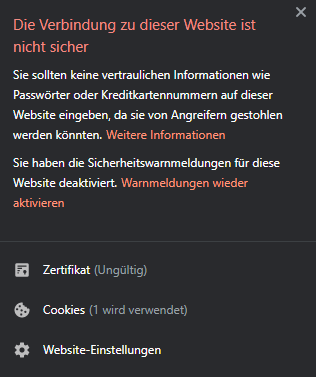
\includegraphics[width=10cm]{not_safe_ssl.png}
\end{center}

\item \textbf{Bruteforce-Angriffe können Datenbank überlasten}

Der Prototyp besitzt keinerlei Zugriffskontrolle. Demnach ist es zum jetzigen Stand möglich, unendlich Anfragen an das Backend zu senden, welches z.B: SQL Anfragen an die Datenbank stellt. Dies könnte die Datenbank überlasten oder sogar den Server crashen. Sollte nämlich kein Pooling mehr möglich sein, wird der Server einen Fehler schmeißen und abstürzen. Dies sollte in einer im Business-Umfeld verwendeten Anwendung implementiert werden, um sowohl den Crash des Servers als auch die Integrität der Daten zu gewährleisten. Ohne solche Abfragen ist das Erraten der Daten des Nutzers (vorallem des Passwortes) nur eine Frage der Zeit und nicht mehr der Möglichkeiten.

\end{enumerate}
